	\documentclass[10pt,oneside]{CBFT_book}
	
	% Algunos paquetes
	
	\usepackage{amssymb}
	\usepackage{amsmath}
	\usepackage{graphicx}
	\usepackage{libertine}
	\usepackage{lipsum}
	\usepackage[numbers]{natbib}
% 	\usepackage{natbib}
	\setcitestyle{square}

	\usepackage{polyglossia}
	\setdefaultlanguage{spanish}


	\usepackage{CBFT.estilo} % Cargo la hoja de estilo

	% Tipografías
	% \setromanfont[Mapping=tex-text]{Linux Libertine O}
	% \setsansfont[Mapping=tex-text]{DejaVu Sans}
	% \setmonofont[Mapping=tex-text]{DejaVu Sans Mono}

	%===================================================================
	%	DOCUMENTO PROPIAMENTE DICHO
	%===================================================================

% \title{CBFT Mecánica clásica}
% \author{Simetrías}
% \date{\today}

\begin{document}
% \maketitle
% \tableofcontents
\chapter{Simetrías}

% =================================================================================================
\section{Constantes de movimiento y simetrías}
% =================================================================================================

Si en las ecuaciones de Euler-Lagrange
\[
	\frac{d}{dt}\left( \dpar{\Lag}{\dot{q}_j} \right) - \dpar{\Lag}{q_j}  = 0, 
\]
se daba el caso de que $ \Lag $ no dependía de $ q_j $ entonces
$ \partial {\Lag} /\partial {q_j}  = 0  $ y
\[
	\frac{d}{dt}\left( \dpar{\Lag}{\dot{q}_j} \right) = 0
\]
significa que 
\[
	\dpar{\Lag}{\dot{q}_j} \equiv p_j
\]
es una constante ($\dot{p}_j=0$).

Por otra parte, si $\delta q_i$ es traslación rígida en una dirección $\hat{n}$ entonces 
\[
	p_i = \vb{P}\cdot\hat{n} \qquad \text{ y } \qquad Q_j= \vb{F}\cdot\hat{n}. 
\]	
En cambio, si $\delta q_i$ es una rotación rígida en torno a un eje $\hat{n}$ se tiene 
\[
p_i = \vb{L}\cdot\hat{n} \qquad  \text{ y } \qquad Q_j= \vb{\Tau}\cdot\hat{n}.
\]

En estos dos casos
\[
	\dpar{T}{q_i} = 0
\]
puesto que:
\begin{itemize}
 \item Como $T$ depende de las velocidades (y no de las coordenadas) no depende del origen y por lo tanto no 
varía ante una traslación rígida (que es un cambio de origen).
 \item Como $T$ es un escalar no cambia ante una rotación.
\end{itemize}

% \[
% 	\dpar{\Lag}{q_i} = 0 = \dpar{T}{q_i} - \dpar{V}{q_i} = 0
% \]
Luego, si $V \neq V(\dot{q})$ (el potencial $V$ no depende explícitamente de las velocidades) entonces las ecuaciones 
de Euler-Lagrange adoptan la forma
% \[
% 	\frac{d}{dt}\left( \dpar{T}{\dot{q}_j} \right) + \dpar{V}{q_j}  = 0 
% \]
\[
	\frac{d}{dt}\left( \dpar{T}{\dot{q}_j} \right) = - \dpar{V}{q_j}   
\]
\[
	\frac{d}{dt}\left( p_j \right) = - \dpar{V}{q_j}   
\]
y entonces 
\[
	\dot{p}_j = -\dpar{V}{q_j}   
\]
es la fuerza total proyectada en la dirección $\hat{n}$.

\notamargen{Acá parecen estar separadas los movimientos rígidos del hecho de que V sea de las coordenadas solamente. 
En un caso tenemos $\dot{p}=0$ y en otro $\dot{p} = -\partial V / \partial q$.
Creo que lo del potencial sería para las otras coordenadas no afectadas por la simetría?.}

Para examinar constantes de movimiento podemos ver primero las variables cíclicas. Sin embargo, si elegimos otras 
coordenadas tal vez no aparezca la constante de movimiento como coordenada cíclica (aunque por supuesto sigue 
existiendo dicha constante).

\subsection{Simetrías en el lagrangiano}

Sea un cambio de coordenadas $q_i \to q_i'$, si como resultado de éste se tenía
\[
	\Lag(q_i, \dot{q}_i, t ) = \Lag(q_i(q_i',t), \dot{q}_i(\dot{q}_i',t), t ),
\]
es decir, que al escribir el lagrangiano en función de las nuevas coordenadas obtengo el mismo, se está ante la 
presencia de una simetría asociada.

Las variables cíclicas son un caso particular de teorema de Noether. Una transformación infinitesimal genérica de $k$ 
grados de libertad es
\begin{eqnarray*}
	q'_1 &= q_1 + \varepsilon g_1(q_1,...,q_k,t) \\
	q'_2 &= q_2 + \varepsilon g_2(q_1,...,q_k,t) \\
	... \\
	q'_k &= q_k + \varepsilon g_k(q_1,...,q_k,t)
\end{eqnarray*}

Para una traslación infinitesimal rígida se tiene 
\begin{eqnarray*}
	x'_i = x_i + \delta x \\
	y'_i = y_i + \delta y \\
	z'_i = z_i + \delta z
\end{eqnarray*}
o bien $\vb{x}' = \vb{x} + \delta \vb{x}$ y la energía cinética 
\[
	T = \sum_i \frac{1}{2} m_i v_i^2
\]
es invariable puesto que depende de las velocidades (que no dependen del origen) y se da $\dot{x} = \dot{x}'$ y lo 
mismo para las otras coordenadas.

Para una rotación en el plano $xy$
\begin{eqnarray*}
	x'_i = x_i + \varepsilon y_i \\
	y'_i = y_i - \varepsilon x_i \\
	z'_i = z_i 
\end{eqnarray*}
que matricialmente se pueden ver como 
\[
	\begin{pmatrix}
	x_i'\\
	y_i'
	\end{pmatrix}
	=
	\begin{pmatrix}
	 1 & \varepsilon \\
	 -\varepsilon & 1
	\end{pmatrix}
	\begin{pmatrix}
	 x_i \\
	 y_i
	\end{pmatrix}
	\qquad 
	\begin{pmatrix}
	 1 & -\varepsilon \\
	 \varepsilon & 1
	\end{pmatrix}
	\begin{pmatrix}
	\dot{x}_i'\\
	\dot{y}_i'
	\end{pmatrix}
	=
	\begin{pmatrix}
	\dot{x}_i \\
	\dot{y}_i
	\end{pmatrix}
\]
resulta
\[
	T = \sum_i \frac{1}{2} m_i v_i^2 = \frac{1}{2} \sum_i m_i ( \dot{x}_i^2 + \dot{y}_i^2 )
\]
y ahora para $T'$ expresamos las coordendas primitivas en función de las nuevas (primadas).
\[
	T' = \frac{1}{2} \sum_i m_i ( [\dot{x}_i' - \varepsilon \dot{y}_i' ]^2 + [\dot{y}_i' + \varepsilon 
\dot{x}_i']^2 )
\]
y a primer orden
\[
	T' = \frac{1}{2} \sum_i m_i ( \dot{x}^{'2}_i - 2 \varepsilon \dot{y}_i'\dot{x}_i' + 
 	2 \varepsilon \dot{y}_i'\dot{x}_i' + \dot{y}^{'2}_i ) = 
 	\frac{1}{2} \sum_i m_i( \dot{x}^{'2}_i + \dot{y}^{'2}_i ) = T.
\]
\notamargen{Resolver un problema de double superscript aquí. T es invariante porque es básicamente un escalar.}

Entonces $T$ es invariante ante traslación rígida y rotación rígida.
Faltaría completar este análisis con las simetrías del potencial $V$ para ver las simetrías del lagrangiano.
En los casos en que 
\[
	V = V(|\vb{x}_i - \vb{x}_j|) \quad \text{ Invariancia de traslación en cualquier dirección} 
\]
lo cual significa depender de la distancia relativa. Otro caso es:
\[
	V = V( x_i, y_i ) \quad \text{ Invariancia de traslación en $z$}
\]

Noether dice que si el lagrangiano $\Lag$ es invariante entonces hay una simetría de la transformación que no 
necesariamente es rotación rígida o traslación rígida.
\[
	T \text{ se conserva en } \begin{cases}
	                           \text{ rotación rígida } \\
	                           \text{ traslaciones }
	                          \end{cases}
\]
\[
	V \text{ tendrá } \begin{cases}
			   \text{ 1. rotación rígida } \\
			    \text{ 2. traslación } \\
			     \text{ 3. rotación y traslación } \\
	                  \end{cases}
\]

Luego, digamos que:
\begin{itemize}
 \item $\Lag$ tiene un momento lineal si $V$ tiene 1
 \item $\Lag$ tiene un momento angular si $V$ tiene 2 
 \item $\Lag$ tiene una combinación de momento lineal y angular si $V$ tiene 3
\end{itemize}

Si se tiene constante de movimiento, no necesariamente el lagrangiano $\Lag$ tiene esa simetría.

Una trasnformación general para $k$ grados de libertad se escribe como 
\begin{eqnarray*}
	q'_1 &= q_1 + \sum_{\ell=1}^S \varepsilon_\ell g_1^\ell(q_1,...,q_k,t) \\
	q'_2 &= q_2 + \sum_{\ell=1}^S \varepsilon_\ell g_2^\ell(q_1,...,q_k,t) \\
	... \\
	q'_k &= q_k + \sum_{\ell=1}^S \varepsilon_\ell g_k^\ell(q_1,...,q_k,t)
\end{eqnarray*}
donde el término en cada sumatoria corresponde al $\delta q_k$.

\notamargen{La simetría de paridad $\vb{x}\to -\vb{x}$, que es una reflexión tiene la particularidad de que es 
discreta, no se puede ir continuamente.}

\subsection{Rotación en 3D infinitesimal}






% =================================================================================================
\section{El teorema de Noether}\index{Noether, teorema de}
% =================================================================================================

Si existe una transformación continua $q_i \longrightarrow q_i + \delta q_i$ que deje invariante el
$\Lag$ entonces hay una constante de movimiento asociada a dicha transformación.

La transformación se puede escribir 
\[
	q_i \longrightarrow q_i' = q_i + \delta q_i
\]
y cumple 
\[
	\Lag(q_i, \dot{q}_i , t) = \Lag(q_i', \dot{q}_i' , t) =
	\Lag(q_i[q_i',t], \dot{q}_i[\dot{q}_i',t] , t)
\]
y así si consideramos una variación a $t$ fijo, también vale que 
\[
	\delta \Lag = \sum_i \dpar{\Lag}{q_i}\delta q_i + \dpar{\Lag}{\dot{q}_i}\delta \dot{q}_i =
	\sum_i \dpar{\Lag}{q_i}\delta q_i + \frac{d}{dt}\left( \dpar{\Lag}{\dot{q}_i}\delta q_i \right)
	- \frac{d}{dt}\left( \dpar{\Lag}{\dot{q}_i} \right) \delta q_i = 0
\]
\[
	\delta \Lag = \sum_i \left[ \dpar{\Lag}{q_i} - \frac{d}{dt}\left( \dpar{\Lag}{\dot{q}_i} \right) \right]
	\delta q_i + \frac{d}{dt}\left( \dpar{\Lag}{\dot{q}_i}\delta q_i \right) = 0
\]
pero como el primer término del RHS es nulo por las ecuaciones de Euler-Lagrange tenemos que 
\[
	\delta \Lag = \frac{d}{dt}\left( \sum_i \dpar{\Lag}{\dot{q}_i}\delta q_i \right)  = 0,
\]
lo que está dentro del paréntesis es la cantidad conservada. 

Existe una simetría (que deja invariante al lagrangiano) y resulta en una constante de movimiento.
No obstante, no toda constante de movimiento proviene de una simetría.

% ~~~~~~~~~~~~~~~~~~~~~~~~~~~~~~~~~~~~~~~~~~~~~~~~~~~~~~~~~~~~~~~~~~~~~~
\begin{ejemplo}{\bfseries Rotación en el plano }

Una rotación en el plano $xy$ bajo un ángulo pequeño $\epsilon$ se puede escribir (ver Apéndice 
\ref{App.rotacion_plana}) como 
\[
 \begin{cases}
  x' = x + \epsilon y \\
  y' = y - \epsilon x
 \end{cases}
\]
\begin{figure}[!htb]
	\begin{center}
	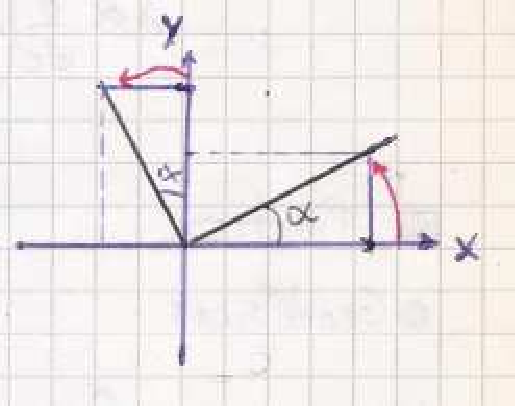
\includegraphics[width=0.35\textwidth]{images/fig_mc_noether1.pdf}	 
	\end{center}
	\caption{}
	\label{fig_mc_noether1}
\end{figure} 

Si consideramos el lagrangiano de una partícula libre en dicho plano $ \Lag = 1/2 m (\dot{x}^2 + \dot{y}^2)$, la 
cantidad conservada será 
\[
	m \dot{x} \delta x + m \dot{y} \delta y = 2\epsilon ( -p_x y + p_y x ) = cte.
\]
que no es otra cosa que el momento angular $L_z$ (que se conserva).

Por supuesto, para una rotación general (no restringida a un plano) son necesarios tres parámetros.
La rotación plana requiere solamente un parámetro.
\end{ejemplo}

% ~~~~~~~~~~~~~~~~~~~~~~~~~~~~~~~~~~~~~~~~~~~~~~~~~~~~~~~~~~~~~~~~~~~~~~

En el caso de una partícula rebotando en un billar hay simetría de rotación en torno a $z$, luego hay
constante de movimiento. En el caso del movimiento elíptico donde 1 y 2 son los focos no hay simetría
de rotación pero aún así hay constante de movimiento $ \ell_1 \ell_2 $.

\begin{figure}[!htb]
	\begin{center}
	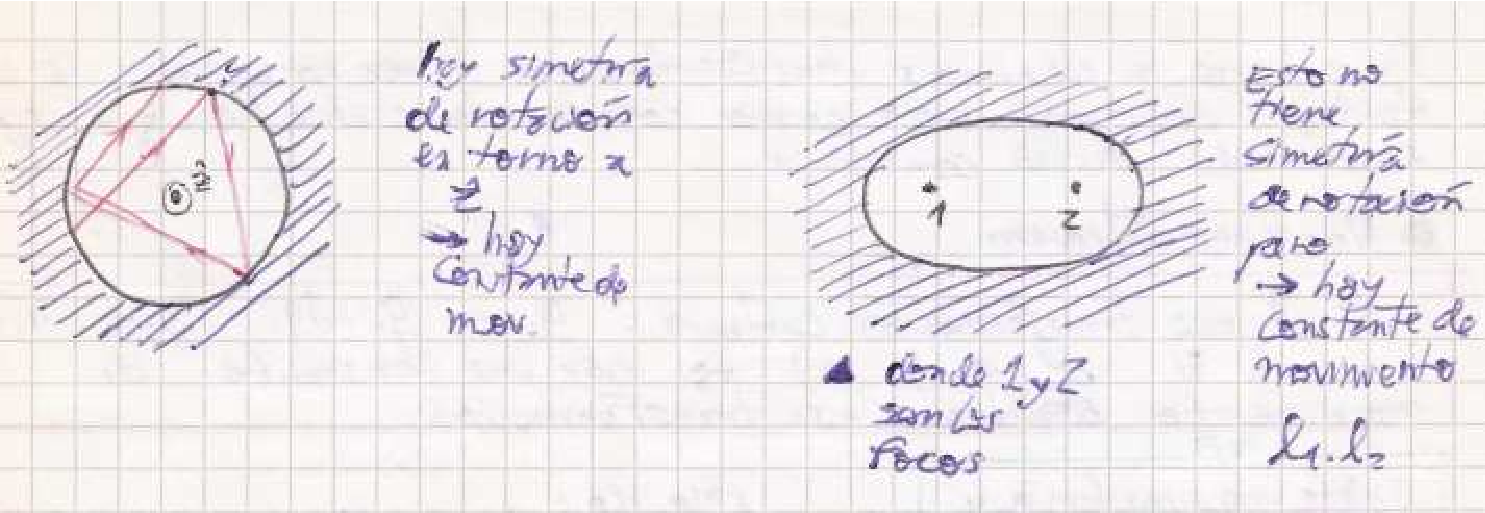
\includegraphics[width=1.0\textwidth]{images/fig_mc_noether2.pdf}	 
	\end{center}
	\caption{}
	\label{fig_mc_noether2}
\end{figure} 

\subsection{Rotación infinitesimal}

\notamargen{En la carpeta estaba este tema. Aparentemente para una rotación general aparecía el momento angular 
conservado, si se manipulaban adecuadamente los índices.}

Recordemos que 
\[
	\delta q_i = q'_i - q_i 
\]
y una traslación infinitesimal es 
\[
	\vb{r}_i' - \vb{r}_i = \delta \vb{r}. 
\]

La variable cíclica es un caso particular de teorema de Noether, pero hay constantes de movimiento que 
no provienen de ninguna simetría.
\[
	\frac{d}{dt}\left( \sum_i \dpar{\Lag}{\dot{q}_i} ( \delta \alpha \hat{n}\times \vb{r}_i ) \right) 
\]
\[
	\frac{d}{dt}\left( \delta\alpha \sum_i \vb{p}_i \times \vb{r}_i  \right) =
	\delta\alpha \frac{d}{dt}\left(  \sum_i \vb{p}_i \times \vb{r}_i  \right) = 0
\]
siendo $\delta \alpha \equiv \epsilon$ un parámetro infinitesimal.
Para $k$ grados de libertad
\begin{align*}
	q'_i &= q_i + \underbrace{\epsilon_i g_i(q_1,...,q_n,t)}_{\delta q} \\
	... \\
	q'_k &= ...
\end{align*}
\[
	\vb{r}_i' = \vb{r}_i + \delta\vb{r} \quad \textrm{traslación rígida}
\]
\[
	\vb{r}_i' = \vb{r}_i + \delta\alpha \; \hat{n}\times\vb{r}_i \quad \textrm{rotación rígida}
\]
o también 
\[
	\delta \vb{r} \times \vb{r}
\]

$T$ es invariante siempre frente a (por ser un escalar)
\[
	T = T' 
\]
entonces habrá que examinarlo.
Constatemos que 
\[
	V = V(|\vb{r}_i - \vb{r}_j|)
\]
es invariancia ante una traslación rígida, y
\[
	V = V(x_1,x_2)
\]
es una invariancia de traslación en $x_3$.

$\Lag$ tendrá como constante un momento lineal si $V$ es invariante frente a traslación.
$\Lag$ tendrá como constante un momento angular si $V$ es invariante frente a rotación.
$\Lag$ tendrá como constante una combinación si $V$ es invariante frente a una roto-traslación.

Otra construcción posible es 
\[
	\delta \Lag = 0
\]
\[
	\Lag( q_i , \dot{q}_i, t ) - \Lag(q_i' , \dot{q}_i' , t) = 0 
\]
pidiendo que $d\Lag = 0$ llego a 
\[
	\sum \left\{ \frac{d}{dt}\left( \dpar{\Lag}{\dot{q}_i} \delta q \right) - 
	\frac{d}{dt}\left( \dpar{\Lag}{\dot{q'}_i} \delta q' \right)  \right\} = 0
\]
\notamargen{Las primas están mal. Hay que pensar una construcción adecuada.
Queda odd.}
\[
	\sum \left\{ \frac{d}{dt}\left( \dpar{\Lag}{\dot{q}_i} \delta q \right) - 
	\frac{d}{dt}\left( \dpar{\Lag}{\dot{q'}_i} \delta q \right) -
	\frac{d}{dt}\left( \dpar{\Lag}{\dot{q'}_i} \sum_\ell^s \epsilon_\ell g_i^\ell \right) \right\} = 0
\]
y podemos usar que 
\[
	\dpar{\Lag}{\dot{q'}_i} = \dpar{\Lag}{\dot{q}_i}
\]
pues $g\neq g(t)$ y es todo a tiempo fijo. Se tiene 
\[
	q' = q + \delta q
\]
\[
	q_i' = q_i + \sum_\ell^s \epsilon_\ell g_i^\ell
\]
siendo esta la transformación general
\[
	\delta q_i' = \delta q_i + \sum_\ell^s \epsilon_\ell g_i^\ell
\]

Extraemos también que 
\[
	\dpar{\Lag}{\dot{q'}_i} \sum_\ell^s \epsilon_\ell g_i^\ell = C
\]

Por hipótesis de Noether, se tiene $\delta \Lag = 0$ y si $\delta$ de la variación es pequeño (o sea que la variación 
es infinitesimal) vale que $d\Lag = 0$. Asimismo, se puede pensar también como que $\Lag$ es invariante ante la 
transformación infinitesimal $\delta q$
\[
	\delta\Lag = \sum_i^N \dpar{\Lag}{q_i}\delta q_i + \dpar{\Lag}{\dot{q}_i}\delta \dot{q}_i = 0
\]
y aplicando la regla de la derivada del producto en el segundo término, se tiene
\[
	\delta\Lag = \sum_i^N \left[ \dpar{\Lag}{q_i} - \frac{d}{dt}\left( \dpar{\Lag}{\dot{q}_i} \right)
	\right]\delta q_i  + \sum_i^N \frac{d}{dt}\left( \dpar{\Lag}{\dot{q}_i} \delta q_i \right)  = 0 
\]
donde el primer término es nulo (por ecuaciones de Euler-Lagrange), y el segundo término 
\[
	\frac{d}{dt} \left( \sum_i^N \dpar{\Lag}{\dot{q}_i} \delta q_i \right)  = 0
\]
involucra la cantidad conservada
\be
	\sum_i^N \dpar{\Lag}{\dot{q}_i} \delta q_i = cte.
	\label{noether_cant_conserv}
\ee

Si se usa la prescripción [de dónde salió?]
\[
	\delta q_i =  \sum_\ell^s \epsilon_\ell g_i^\ell(q_1,q_2,...,q_n)
\]
en \eqref{noether_cant_conserv} se tiene 
\[
	\frac{d}{dt} \left( \dpar{\Lag}{\dot{q}_1} \sum_{\ell=1}^s \epsilon_\ell g_1^\ell  + 
	\dpar{\Lag}{\dot{q}_2} \sum_{\ell=1}^s \epsilon_\ell g_2^\ell + ...	
	\right)  = 0
\]
y si tomo $epsilon_1 =\epsilon$ y todos los $\epsilon_2,\epsilon_3,...=0$ lo cual se puede hacer puesto que son 
independientes,
\[
	\frac{d}{dt} \left( \dpar{\Lag}{\dot{q}_1} \epsilon g_1^1  + 
	\dpar{\Lag}{\dot{q}_2} \epsilon g_2^1 + ...	\right)  = 0
\]
y como los primeros términos dentro de cada sumando en el paréntesis son los momentos canónicamente conjugados,
\[
	\frac{d}{dt} \left( \sum_i p_i g_i^1 \right)  = 0
\]
\[
	\frac{d}{dt} \left( \sum_i p_i g_i^2 \right)  = 0
\]
\[
	\frac{d}{dt} \left( \sum_i p_i g_i^\ell \right)  = 0 \qquad \ell =1,2,...,s
\]
y tendré una constante de movimiento por cada parámetro independiente.
\notamargen{Acá no entiendo bien de qué la va esta construcción.}

\subsection{Rotación en 3D infinitesimal}

En este caso se escribe 
\[
	\vb{x}_i' = \vb{x}_i + \delta \: \hat{n}\times\vb{x}_i
\]
que es una rotación en torno a un versor genérico $\hat{n}$ y el carácter de infinitesimal viene dado por $\delta \ll 
1$.
En términos de coordenads esféricas
\[
	(\sin\theta\cos\phi,\sin\theta\sin\phi,\cos\theta)\times (x_i,y_i,z_i)
\]
de modo que 
\begin{eqnarray*}
	x_i' = x_i + \delta( \sin\theta \sin\phi z_i - \cos\theta y_i ) &\\
	x_i' = x_i + \delta( \cos\theta x_i - \sin\theta\cos\phi z_i ) &\\
	x_i' = x_i + \delta( \sin\theta \cos\phi y_i - \sin\theta\sin\phi x_i ) &
\end{eqnarray*}
que es una rotación controlada por tres parámetros ($\theta,\phi,\delta$).
Como por hipótesis la rotación es una trasnsformación de simetría se tendrá
\[
	\dtot{}{t}\left( \sum_i \dpar{\Lag}{\dot{x}_i} \delta x_i +  
	\dpar{\Lag}{\dot{y}_i} \delta y_i +
	\dpar{\Lag}{\dot{z}_i} \delta z_i \right) = 0
\]
y si usamos las expresiones dadas por las ecuaciones anteriores donde $\delta$ es una constante, se tendrá
\[
	\delta \cdot \dtot{}{t}\left( \sum_i ( p_{x_i} z_i - p_{z_i}x_i )\sin\theta\sin\phi + 
	( -p_{x_i} y_i + p_{y_i} x_i )\cos\theta + ( -p_{y_i} z_i + p_{z_i} y_i )\sin\theta\cos\phi \right) = 0
\]
y como $\theta,\phi,\delta$ son independientes tomo $\theta=0$ y $\phi$ genérico para llegar a
\[
	\delta \cdot \dtot{}{t}\left( \sum_i ( p_{y_i} x_i - p_{x_i} y_i ) \right) = 0
\]
que implica $L_z$ constante. De forma similar, considerando $\theta=\pi/2$ y $\phi=0$
\[
	\delta \cdot \dtot{}{t}\left( \sum_i ( p_{z_i} y_i - p_{y_i} z_i ) \right) = 0,
\]
que conduce a $L_x$ constante. Finalmente, $\theta=\pi/2$ y $\phi=\pi/2$ desemboca en $L_y$ constante,
\[
	\delta \cdot \dtot{}{t}\left( \sum_i ( p_{x_i} z_i - p_{z_i} x_i ) \right) = 0.
\]

\notamargen{Tener en cuenta que conservamos el $L$ total, i.e. la $\sum_i$. }

\begin{ejemplo}{\bf Helicidad}

Supongamos una transformación
\begin{eqnarray*}
	&\rho' = \rho \\
	&z' = z + a \delta \vp \\
	&\vp' = \vp + \delta\vp 
\end{eqnarray*}
que es una rotación y traslación. Automáticamente $T$ es invariante ante tal transformación y según Noether se conserva
\[
	\sum_i \dpar{\Lag}{\dot{\vp}_i} \delta \vp + \sum_i \dpar{\Lag}{\dot{z}_i} a \delta \vp +
	\sum_i \dpar{\Lag}{\dot{\rho}_i} 0 = cte.
\]
\[
	\sum_i l_{z_i} + a \sum_i p_{z_i}  = \sum_i \left( l_{z_i} + a p_{z_i} \right) = \frac{cte. }{\delta \vp}
\]
y la cantidad entre paréntesis es la helicidad.
\end{ejemplo}

El caso más general es cuando
\[
	\Lag(q) = \Lag{\dot{q}} + \varepsilon \dtot{f}{t}
\]
y entonces
\[
	\sum p_i \delta q_i + f
\]
esta forma toman las constantes de movimiento.
\notamargen{Corregir esto!}

\begin{ejemplo}{\bf Resortes enganchados}

Este es el problema 1.
 
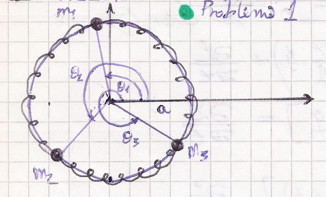
\includegraphics[scale=0.3]{images/fig_mc_resortes.jpg} 

\[
	T = \frac 1 2 m_1 a^2 \dot{\theta}_1^2 + \frac 1 2 m_2 a^2 \dot{\theta}_2^2 + \frac 1 2 m_3 a^2 \dot{\theta}_3^2
\]
\[
	V = \frac k 2 (\theta_1 -\theta_2 )^2 + \frac k 2 (\theta_2 -\theta_3 )^2 + \frac k 2 (\theta_3 -\theta_1 )^2
\]
Sería de esperar que en este caso se conserven algunas cosas y que sean visibles esas conservaciones observando 
simetrías.

Una manera de explicitar esto sería expresar $V$ en función de nuevas coordenadas, así el lagrangiano no dependerá de 
alguna [?]
\[
	q_1 =\theta_1 -\theta_2 \qquad q_2 = \theta_2 -\theta_3 \qquad q_3 = \theta_3
\]
y con estas definiciones
\[
	q_1+q_2 = \theta_1-\theta_3 
\]
y será $V=V(q_1,q_2)$. Entonces 
\[
	p_3 = \dpar{\Lag}{\theta_3} = cte
\]
\notamargen{Esta es la manera formal de generar estas conservaciones [?].}
Esto era de esperar nomás mirar el sistema; tenía una simetría de rotación.
\end{ejemplo}

\begin{ejemplo}{\bf Rotación en cilindros [¿?]}

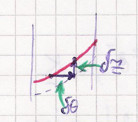
\includegraphics[scale=0.4]{images/fig_mc_simetria_rot2.jpg}

Si roto en $\vp$ el potencial no ve cambios. Entonces una variación en el lagrangiano toma la forma
\[
	\delta \Lag = \dpar{\Lag}{\vp}\delta\vp = L\vp \delta\vp = 0
\]

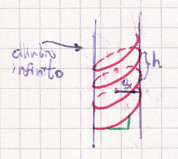
\includegraphics[scale=0.4]{images/fig_mc_simetria_rot1.jpg}

Si varío en $z$ y en $\vp$ la transformación
\[
	\delta \Lag = \dpar{\Lag}{z}\delta z + \dpar{\Lag}{\vp}\delta\vp = 0
\]
será nula. Si elegimos las coordenadas usuales para este problema,
\[
	x = a \cos \theta \qquad y = a \sin \theta \qquad z = \frac{h\theta}{2\pi}
\]
A partir de
\[
	\dtot{}{t}\left( \dpar{\Lag}{\dot{z}} \right)\delta z + \dtot{}{t}\left( \dpar{\Lag}{\dot{z}} \right)\delta\vp,
\]
se puede {\it amasar} la expresión para llegar a
\[
	\left( \dot{p}_z  \frac{h}{2\pi} + L_\vp \right) \delta \vp
\]

\notamargen{Estoy buscando una simetría del potencial girando en $2\pi$.}

 
\end{ejemplo}

\begin{ejemplo}{\bf Secciones cónicas}
 
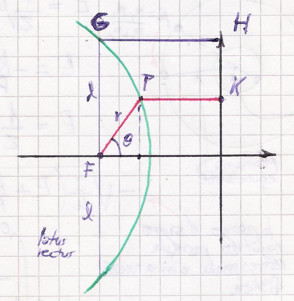
\includegraphics[scale=0.3]{images/fig_mc_secciones_conicas.jpg} 
 
La sección cónica es el lugar geométrico que cumple 
\[
	\bar{PF} = e \bar{PK}
\]
donde $0 \leq e \leq +\infty$ y se tiene
\[
	\begin{cases}
	e < 1 \quad \text{ elipse } \\
	e = 1 \quad \text{ parábola } \\
	e > 1 \quad \text{ hipérbola }
	\end{cases}
\]
\[
	PF = e (GH - PF \cos\theta ) \qquad PF(1-e\cos\theta) = e GH
\]
\[
	r(1-e\cos\theta)=\ell
\]

Si $e<1$ se da
\[
	\frac{ x - e\ell/(e^2-1)}{a^2} + \frac{y^2}{b^2}= 1 \qquad a^2 = \left( \frac{\ell}{e^2-1} \right)^2 
\]
Si por el contrario es $e>1$
\[
	\frac{ x - e\ell/(e^2-1)}{a^2} - \frac{y^2}{b^2}= 1 \qquad b^2 = \left( \frac{\ell}{\sqrt{e^2-1}} \right)^2 
\]
Si el origen de coordenadas está en el foco.
\end{ejemplo}


\begin{ejercicios}

\label{ej1}
\item{ \bf }
Sean tres masas m1 , m2 y m3 , enhebradas en un aro circular fijo. Las masas interactúan
a través de ciertos resortes especiales cuyo potencial es V (θi , θj ) = 21 k(θi − θj )2 , donde
i, j = 1, 2, 3 y k es una constante. En base a la simetrı́a del lagrangiano —teorema de
Noëther— hallar qué magnitudes se conservan.

\label{ej2}
\item{ \bf }
Qué componentes de p y L se conservan para el movimiento de una partı́cula en los
siguientes campos?
\begin{enumerate}[label=(\alph*)]
\item Los podetneciales son constantes sobre superficies elipsoidales (a 6= b 6= c).
\item Las superficies equipotenciales son planos homogéneos infinitos.
\item Las superficies equipotenciales son cilindros infinitos.
\item De simetrı́a helicoidal.
\item Campo debido a una red unidimensional de cargas positivas separadas entre sı́
una distancia d constante.
\item Las superficies equipotenciales son toros.
\end{enumerate}


\label{ej3}
\item{ \bf }
Cómo serı́an las órbitas de los planetas si el potencial gravitatorio solar tuviera simetrı́a
cilı́ndrica?.


\label{ej4}
\item{ \bf }
Se tienen dos partı́culas de masa m1 y m2 que interactúan con un potencial V =
V (r1 − r2 ). Demuestre explı́citamente que para que se conserve el impulso angular es
necesario que V = V (|r1 − r2 |).


\label{ej5}
\item{ \bf }
Calcule las constantes de movimiento para una partı́cula en el espacio, en un campo
electromagnético, con potenciales:
\begin{enumerate}[label=(\alph*)]
\item  φ = φ(x, y) ; A = A(x, y)b z
\item  φ = φ(x2 + y 2 , z) ; A = A(x2 + y 2 , z)b
\end{enumerate}

\end{ejercicios}



% =================================================================================================
% 

% \bibliographystyle{CBFT-apa-good}	% (uses file "apa-good.bst")
% \bibliography{CBFT.Referencias} % La base de datos bibliográfica

\end{document}
